\documentclass[letterpaper, 8pt]{extarticle}
\usepackage{amssymb,amsmath,amsthm,amsfonts}
\usepackage{multicol,multirow}
\usepackage{calc}
\usepackage{ifthen}
\usepackage[landscape]{geometry}
\usepackage[colorlinks=true,citecolor=blue,linkcolor=blue]{hyperref}
\usepackage{booktabs}
\usepackage{ulem}
\usepackage{enumitem}
\usepackage{tabulary}
\usepackage{graphicx}
\usepackage{siunitx}
\usepackage{tikz}
\usepackage{derivative}
\usepackage{svg}
\usepackage{listings}
\usepackage{color}
\usepackage{soul}
\usepackage{clrscode3e}


\ifthenelse{\lengthtest { \paperwidth = 11in}}
    { \geometry{top=.25in,left=.25in,right=.25in,bottom=.3in} }
	{\ifthenelse{ \lengthtest{ \paperwidth = 297mm}}
		{\geometry{top=1cm,left=1cm,right=1cm,bottom=1cm} }
		{\geometry{top=1cm,left=1cm,right=1cm,bottom=1cm} }
	}

\newenvironment{Figure}
  {\par\medskip\noindent\minipage}
  {\endminipage\par\medskip}

\pagestyle{empty}
\makeatletter
\renewcommand{\section}{\@startsection{section}{1}{0mm}%
                                {-1ex plus -.5ex minus -.2ex}%
                                {0.5ex plus .2ex}%x
                                {\normalfont\normalsize\bfseries}}
\renewcommand{\subsection}{\@startsection{subsection}{2}{0mm}%
                                {-1explus -.5ex minus -.2ex}%
                                {0.5ex plus .2ex}%
                                {\normalfont\small\bfseries}}
\renewcommand{\subsubsection}{\@startsection{subsubsection}{3}{0mm}%
                                {-1ex plus -.5ex minus -.2ex}%
                                {1ex plus .2ex}%
                                {\normalfont\tiny\bfseries}}
\makeatother
\setcounter{secnumdepth}{0}
\setlength{\parindent}{0pt}
\setlength{\parskip}{0pt plus 0.5ex}
% -----------------------------------------------------------------------
% \tymin=37pt
% \tymax=\maxdimen

% Custom siunitx defs
\DeclareSIUnit\noop{\relax}
\setlist[itemize]{noitemsep, leftmargin=*}
\setlist[enumerate]{noitemsep, leftmargin=*}

\NewDocumentCommand\prefixvalue{m}{%
\qty[prefix-mode=extract-exponent,print-unity-mantissa=false]{1}{#1\noop}
}

% Shorthand definitions
% \newcommand{\To}{\Rightarrow}

% condense itemize & enumerate
\let\olditemize=\itemize \let\endolditemize=\enditemize \renewenvironment{itemize}{\olditemize \itemsep0em}{\endolditemize}
\let\oldenumerate=\enumerate \let\endoldenumerate=\endenumerate \renewenvironment{enumerate}{\oldenumerate \itemsep0em}{\endoldenumerate}

\title{2GA3}

\begin{document}

\raggedright
\tiny

\begin{center}
	{\textbf{2GA3}} \\
\end{center}
\begin{multicols*}{4}
	\setlength{\premulticols}{1pt}
	\setlength{\postmulticols}{1pt}
	\setlength{\multicolsep}{1pt}
	\setlength{\columnsep}{2pt}

	\section{Logic Basics}
	% \subsection{Physics}
	% \textbf{Ohm's Law:} $R = \frac{U}{T}$\\
	% \textbf{Series:} \\
	% $R_T = \sum_{i=1}^N R_i$ \\
	% $V_T = \sum_{i=1}^N V_i$ \\
	% $I_T = I_1 = I_2 = \dots = I_N$\\
	% \textbf{Parallel:} \\
	% $1/R = \sum_{i=1}^N (1/R_i)$\\
	% $V_T = V_1 = V_2 = \dots = V_N$\\
	% $I_T = \sum_{i=1}^N I_i$ \\

	\subsection{Transistors}
	MOSFETs have 4 components: Source, Gate, Drain, and Base

	\textbf{PNP/NMOS:} Is on when gate is positive. No circle. \\
	\textbf{NPN/PMOS:} Is on when gate is negative. Has circle.

	Generally, transistors are used to pull the output to either
	a positive voltage, or a zero voltage (1 or 0, on or off).
	If output is not pulled to one of these,
	the output is floating and is indeterminate in voltage.

	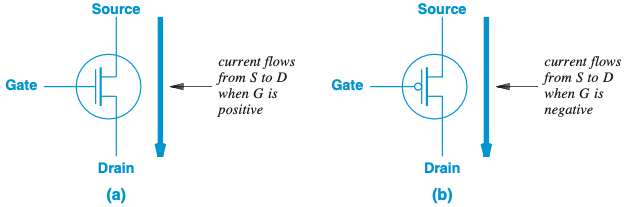
\includegraphics[width=\linewidth]{transistor-types.png}

	\subsection{Logic Circuits}
	\subsubsection{Symbols}

	\begin{center}
		\begin{tabular}{@{}ll|llllll@{}}
			\toprule
			p & q & and & nand & or & nor & xor & invert p \\
			\midrule
			1 & 1 & 1   & 0    & 1  & 0   & 0   & 0         \\
			1 & 0 & 0   & 1    & 1  & 0   & 1   & 0         \\
			0 & 1 & 0   & 1    & 1  & 0   & 1   & 1         \\
			0 & 0 & 0   & 1    & 0  & 1   & 0   & 1         \\
			\bottomrule
		\end{tabular}
	\end{center}

	\begin{center}
		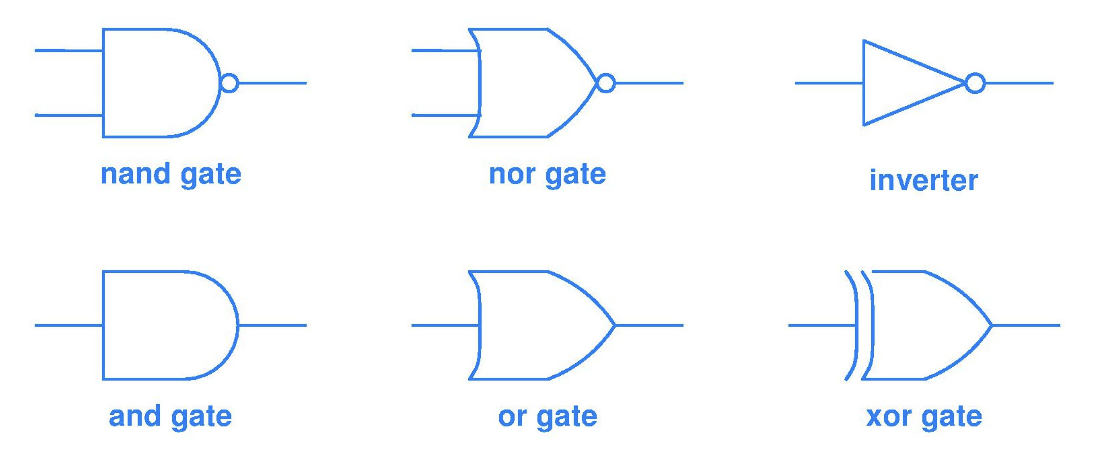
\includegraphics[width=.8\linewidth]{logic-gates.png}
	\end{center}
	\subsubsection{Adders}
   Left: Half-adder. Right: Full-adder.
	\begin{center}
		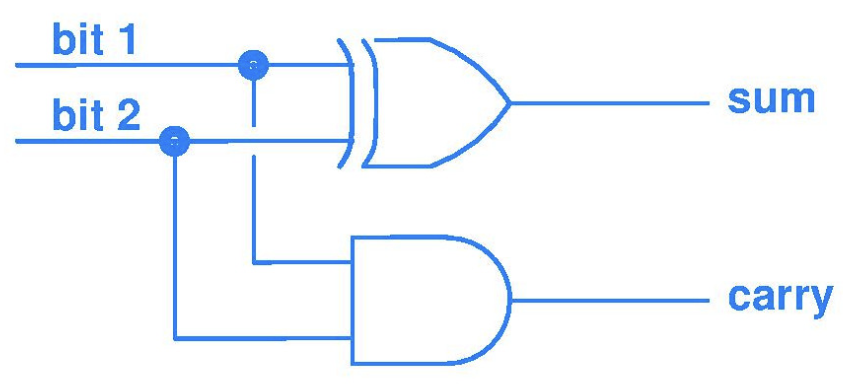
\includegraphics[width=.5\linewidth]{half-adder.png} \\
		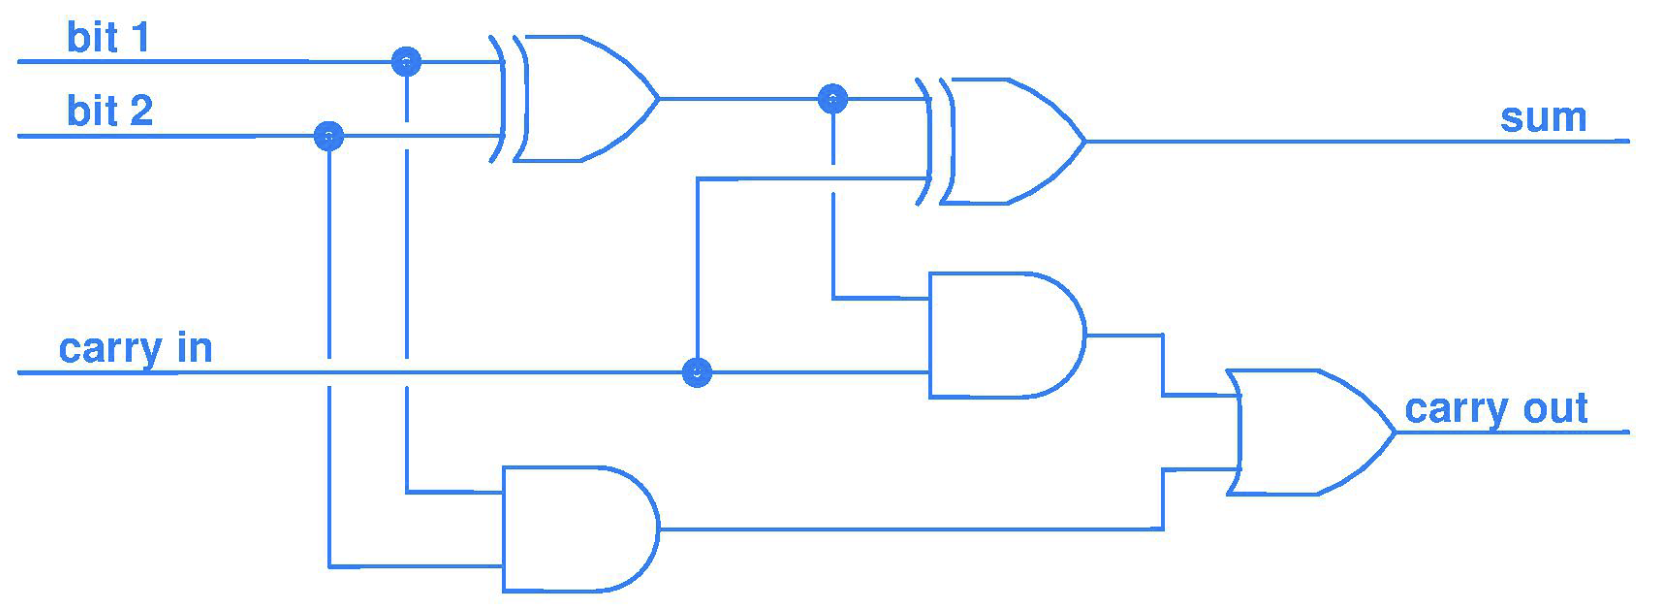
\includegraphics[width=.9\linewidth]{full-adder.png} \\
		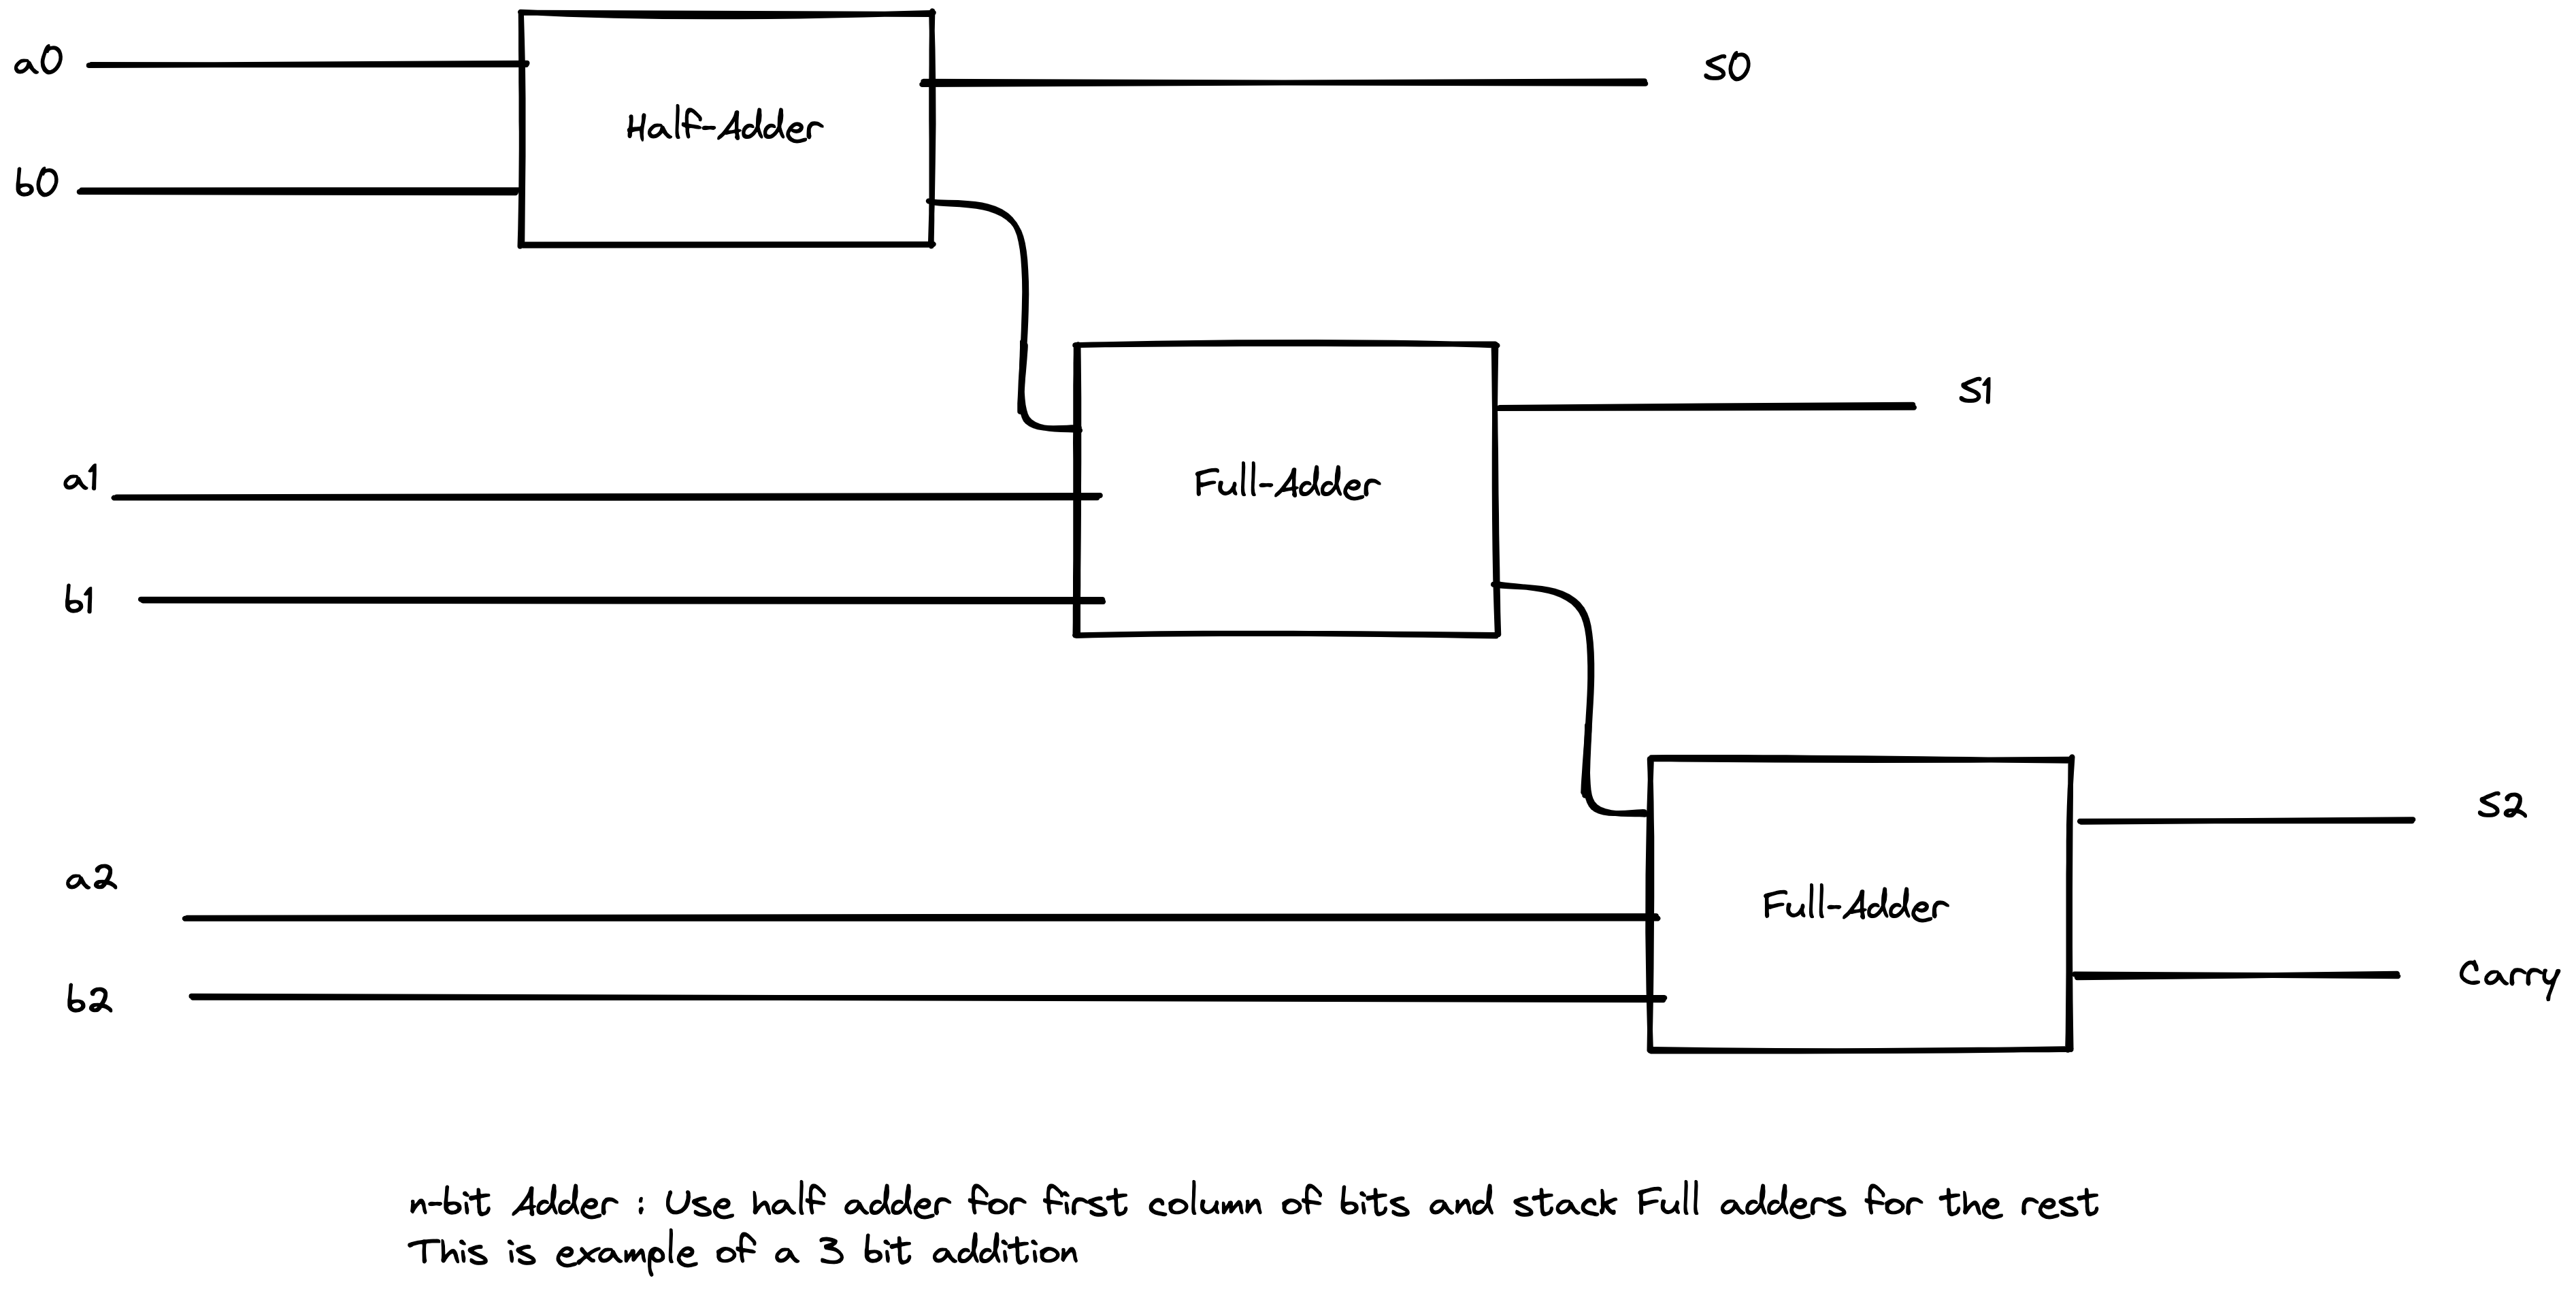
\includegraphics[width=0.8\linewidth]{n-adder.png}
	\end{center}
	% REVIEW: Is there anything else that needs to be added here?
	Unlike half-adders, full-adders can recieve carry-in bits.
	To add more bits, chain multiple full-adders together.
	If final carry at end is 1, there's an overflow error.

	\subsubsection{Latches \& Flip-flops}
	\textbf{Flip-flop}
	Every time the input switches from 0 to 1, the output switches to
   the opposite.
	% TODO: Add more detail about flip-flops

	\textbf{Gated D-latch} \\
	\begin{center}
		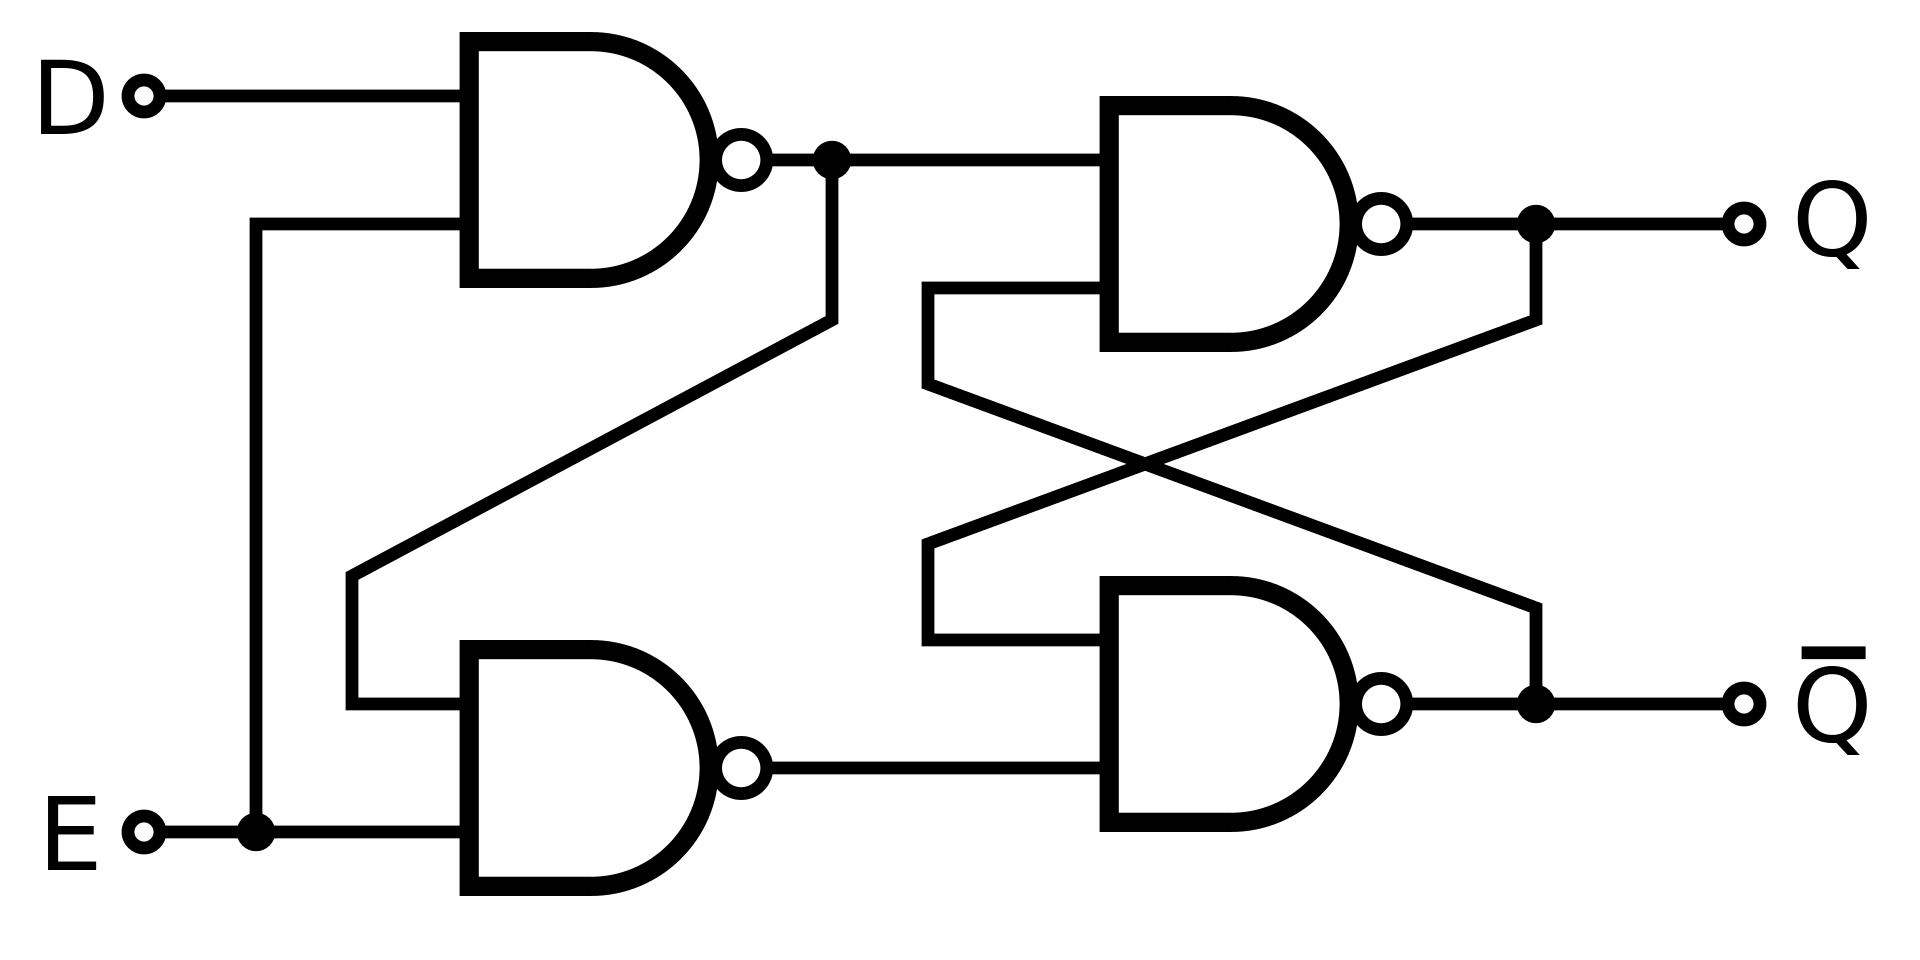
\includegraphics[width=.6\linewidth]{gated-d-latch.png}
		\begin{tabular}[!ht]{@{}cc|ccc@{}}
			\toprule
			$E/C$ & $D$ & $Q$               & $\overline{Q}$               & Comment   \\
			\midrule
			0     & X   & $Q_\textit{prev}$ & $\overline{Q}_\textit{prev}$ & No change \\
			1     & 0   & 0                 & 1                            & Reset     \\
			1     & 1   & 1                 & 0                            & Set       \\
			\bottomrule
		\end{tabular}
	\end{center}
	\begin{itemize}
      \item Q - The stored bit
      \item D - Data/bit to write to Q
      \item E - The enabler (Must be 1 to enable writing, otherwise nothing changes)
      \item Operate on the principle of propagation delay.
      \item Stacking many of them can be used to create a register:
   \end{itemize}

	% REVIEW: Do we need this?
	% seems like a lot of space dedicated to something that's trivial to derive
	% from scratch
	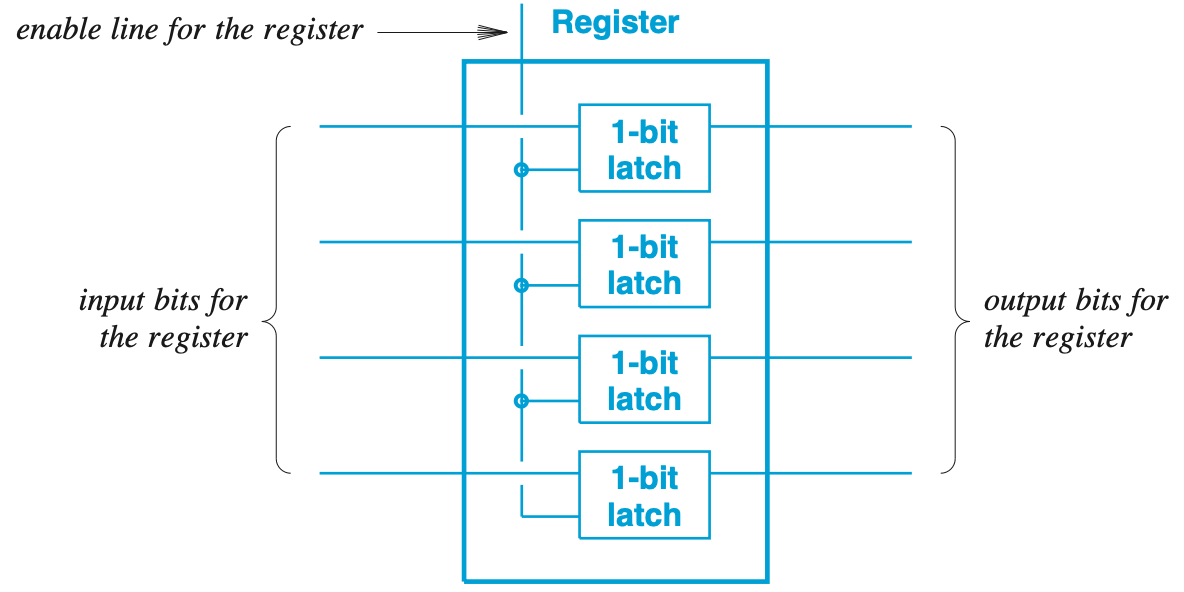
\includegraphics[width=\linewidth]{register.png}

	\subsection{Counters}
	For each transition from \textbf{low to high}, the counter increments
   the binary output by 1. (Counting the transition from high to low does
   the same thing, but the lecture used rising-edge counters).

	\subsection{Decoders}
	Take in an $n$-bit number, and turn on one of $2^n$ outputs.

	\subsection{Multiplexer / Demultiplexer}
	\textbf{Multiplexer} turns $n$ signals into a single signal. Chooses
   which signal to let through. \textbf{Demultiplexer} turns a single signal
   into $n$ signals. The single signal chooses which signal to output.

	\subsection{Software vs Hardware Design}
	Unlike software, which uses iteration, hardware uses replication. The advantages of replication are increased elegance, higher speed, and increased reliability.
	Hardware also uses gate minimization, abstraction and power optimization.

	\subsection{Fixed \& Programmable Logic}
	\textbf{Fixed logic circuits:} Pre-determined function.
	\textbf{Programmable logic:} FPGAs (reprogrammable, but still a significant cost to switching functions).
	\textbf{Stored program and re-programmable circuits:} Your computer right now.
	\section{Data Encoding}
	1 Byte = 8 bits.
	1 \textbf{Byte} encodes a character, integer, or pointer.
	1 \textbf{Word} is $n$ bytes, determined by the architecture.

	\subsection{Converting between bases}
	\textbf{Base 10 to Base N}
	Divide decimal \# by \# of new base.
	Take remainder as rightmost digit.
	Divide quotient of previous divide by new base.
	Repeat until quotient is zero.
	\textbf{Base N to Base 10}
	Take each column position of each digit, zero indexed, as $n$.
	For each column, do $c \cdot b^n$, where $c$ is the value of the column,
	and $b$ is the base value in base 10.

	% REVIEW: if anyone can explain this better feel free to update this
	\subsection{Fraction to Binary}
   \begin{itemize}
      \item Let $x$ be the decimal part of our fraction.
      \item Let $b$ be our binary output
      \item Multiply $x$ by 2.
      \item If $x \geq 1$, subtract 1 from $x$ and append 1 to $b$.
      \item If $x < 1$, append 0 to $b$.
      \item Repeat until $x != 0$.
   \end{itemize}

	\subsection{Signed Integers}
	\textbf{Sign-magnitude:} Dedicate one bit to the sign, and the rest to the magnitude.
	Range is $-(2^{n-1} - 1), +(2^{n-1} - 1)$,
	but has a positive and negative zero.
	\textbf{One's complement:} Invert all the bits to get negative number.
	Range is $-(2^{n-1} - 1), +(2^{n-1} - 1)$.
	\textbf{Two's complement:} Invert all bits, add a place value of 1 to get negative number.
	Eg, +6 is $0110$, so to get -6 go from $0110 \to 1001 \to 1010$.
	Range is $-(2^{n-1}), +(2^{n-1} - 1)$.

	\subsection{IEEE-754 Floats}
	Separated into \textbf{sign, exponent, and mantissa}.
	Entire float is represented in binary, and the exponent is biased by $2^{b-1} - 1$,
	where $b$ is the number of exponent bits.
	To calculate from IEEE, do $m_2 \times 2^{e_2}$.
	(Convert out of base 2 first).
	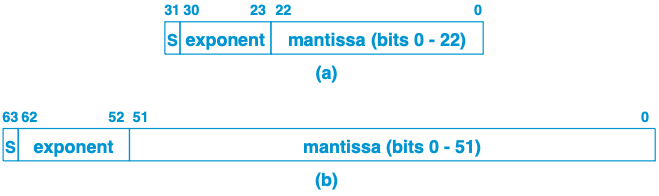
\includegraphics[width=\linewidth]{ieee-754.png}

	\subsubsection{Special Values}
   \begin{center}\begin{tabular}[!ht]{@{}cc|c@{}}
      \toprule
      Exponent & Mantissa & Value \\
      \midrule
      all 1s   & all 0s   & $\pm \infty$ \\
      all 1s   & not all 0s & NaN \\
      all 0s   & not all 0s & denormalized \\
      all 0s   & all 0s   & $\pm 0$ \\
      \bottomrule
   \end{tabular}\end{center}

	\subsection{Types of architecture}
	\textbf{Von Neumann architecture:}
	\begin{itemize}
		\item Single memory block which contains both instructions and data.
		\item Offers complete flexibility: at any time, owner can change how much of the memory is devoted to programs and how much to data.
		\item More popular.
	\end{itemize}
	\textbf{Harvard architecture:}
	\begin{itemize}
		\item 2 separate memory. One is used for instruction, one is used for data.
		\item Inflexible, as u cannot use part of the instructional memory to store data and vise versa.
		\item Less popular. Sometimes used in small embedded systems.
	\end{itemize}

	\subsection{Types of processors}

	\textbf{Categories based on logic:} \\
	\begin{itemize}
		\item \textbf{Fixed logic}: Function fixed in hardware, performs a single task
		\item \textbf{Selectable logic}: Choose one of several fixed functions.
		\item \textbf{Parametrizable logic}: Accepts a set of parameters that control the computation of fixed functions.
		\item \textbf{Programmable logic}: list of instructions provided at runtime (you can code them)
	\end{itemize}

	\textbf{Categories based on Complexity:} \\
	\begin{itemize}
		\item \textbf{Co-processors}: Dedicated function. Usually performs a single task at high speed. Fixed/Selectable logic.
		\item \textbf{Microcontrollers}: Direct hardware control. Used in -> Elevator doors. Programmable logic.
		\item \textbf{Embedded System Processors}: real-time OS, dedicated hardware. usually more powerful than microcontrollers. Used in -> smart phone Programmable logic.
		\item \textbf{General-purpose Processors}: compatible for multiple systems. Used in -> CPU in a PC. Programmable logic.
	\end{itemize}

	\subsection{Parts of a processor}
	\begin{itemize}
		\item \textbf{Controller}: Responsible for program execution. Steps through the program and coordinates the actions of all other units.
		\item \textbf{Arithmetic logic unit}: Performs all computational tasks. Performs one operation at a time according to controller.
		\item \textbf{Local storage (registers)}: Hold data values such as operands for arithmetic operations and the result.
		\item \textbf{Internal connections}: Transfers data values between units, like from local storage to the ALU. AKA data paths/Bus/Control lines
		\item \textbf{External interface}: Handles all communication between the processor and the rest of the computer system.
	\end{itemize}

	\subsection{Fetch execute cycle}
	There is a \textbf{instruction pointer} which moves through the program performing every step. The cycle never ends while the system is runing.
	\begin{itemize}
		\item Fetch the next instruction
		\item Decode the instruction and fetch operands from registers
		\item Perform the arithmetic operation specified by the \textbf{opcode}
		\item Perform memory read or write, if needed
		\item Store the result back to the registers
		\item go to next instruction, Repeat forever.
	\end{itemize}

	\subsection{Program Translation}
	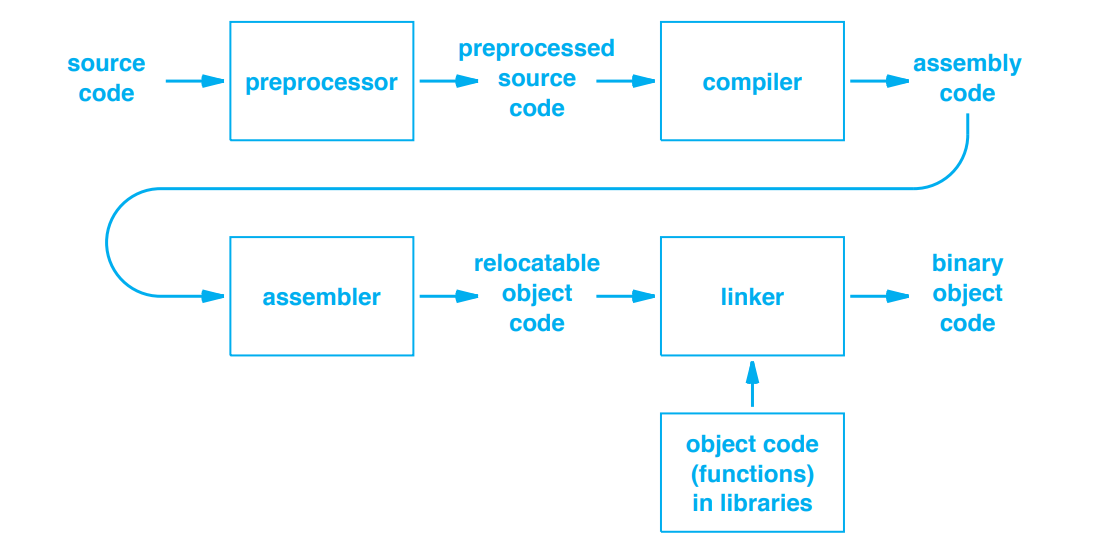
\includegraphics[width=\linewidth]{program-translation.png}
	\begin{itemize}
		\item \textbf{Preprocessor:} Expands macros, producing modified source program.
		\item \textbf{Compiler:} Translates it to assembly.
		\item \textbf{Assembler:} Translates it to relocatable object code which contains references to external library functions.
		\item \textbf{Linker:} Replaces external function references with its code.
	\end{itemize}

	\subsection{CISC vs RISC}
	\textbf{CISC}
	\begin{itemize}
		\item Each instruction performs a complex operation
		\item Instructions may take multiple clock cycles
		\item Fewer instruction calls
	\end{itemize}
	\textbf{RISC}
	\begin{itemize}
		\item Each instruction performs a simple operation
		\item Instructions all take the same number of clock cycles
		\item Many instruction calls needed
		\item Allows for pipelining, as each part of the instruction takes the same amount of time
	\end{itemize}

	\subsection{Pipelines}
	Allow for more than one instruction to be ``processed'' at the same time.
	Generally 5 stages:
   \begin{enumerate}
      \item Fetch next instruction
      \item decode \& fetch operands
      \item perform arithmetic operation
      \item read or write memory
      \item store result
   \end{enumerate}

	\subsubsection{Pipeline Stalls}
	Also known as hazards. 3 main types:
   \begin{itemize}
      \item
         \textbf{Data Hazards:} Waiting for data from an earlier instruction.
         Can be dealt with using data forwarding (allowing data to be used
         before it exits the pipeline), re-arranging instruction order.
      \item
         \textbf{Control Hazards:} Incorrect instruction is in the pipeline.
         Occurs during jump instructions/branching. Jumps are not executed
         until the fifth stage, so instructions directly after are fetched
         inside the pipeline.  Can be dealt with using conditional branch
         prediction, flushing pipeline if prediction is wrong.
      \item
         \textbf{Structural Hazards:} Resource conflict (usually from external
         source) (eg sombody else is accessing the same register bank). Can
         be dealt with by loading data in parallel, eg using multiple banks.
   \end{itemize}

	\subsection{Branching}
	Moving the instruction pointer to a different location in program.
	Can be either absolute branch, or relative branch.
	% REVIEW: idk what else needs to be added here,
	% this seems pretty trivial

	\section{Instruction Sets}
	Generally has the following parts:
	Operation number, registers, offset.
	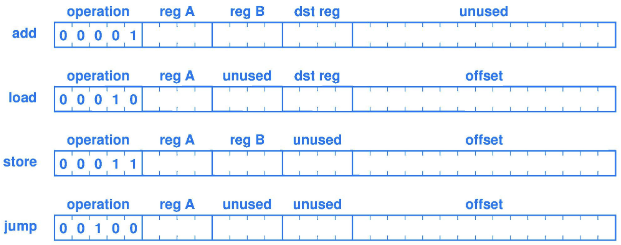
\includegraphics[width=\linewidth]{isa-example.png}

	\subsection{Design choices}
	\subsubsection{Encoding length}
	\textbf{Variable-length} encoding can improve instruction density,
	but \textbf{fixed-length} instructions are simpler to implement in hardware,
	and are thus more performant. Unused bits are ignored by the instruction.

	Offsets are used to encode immediate values (generally used for jumping).

	\subsubsection{Number of Operands}
	\textbf{Zero operands:} Stack architecture, using push and pop. All operands are implicit.
	\textbf{One operand:} Implicit destination (usually a special accumulator register)
	\textbf{Two operands:} Specified destination, but uniary operations (eg \verb|add rA, rB #rA=rA+rB|)
	\textbf{Three operands:} Specified destination, binary operations
	TL;DR, more operands = more flexible instructions, but more space taken up by operands

	\subsubsection{Implicit vs Explicit Encoding}
	\textbf{Implicit Encoding:} Operand types are always the same for a given opcode.
	Different opcodes are used for different types.
	\textbf{Explicit Encoding:} Operand field specifies what type of operands are being provided.

	\subsubsection{Operand Adressing Modes}
	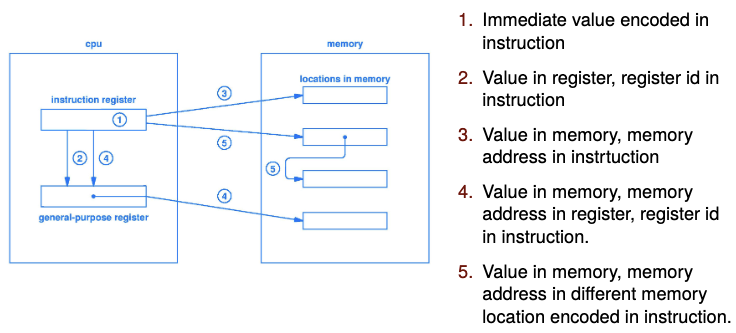
\includegraphics[width=\linewidth]{operand-addressing-modes.png}

	\subsubsection{Orthogonality}
	Each instruction should perform a \textit{unique task},
	without duplicating or overlapping the functionality of other instructions.
	Advantages: Orthogonal instructions can be understood more easily,
	and programmers don't need to pick between functions that perform the same task.

	\subsection{Registers}
	\textbf{General Registers}
	Fixed size (usually 32 or 64 bits), 2 basic ops, fetch and store.
	Numbered from 0 to $N-1$.
	\textbf{Floating Point Registers}
	Separate set of registers holding floats, but numbering overlaps.
	Floating point registers are automatically used if instruction requires FP.
	\textbf{Special Registers}
	The program counter (\textit{pc}) and accumulator (\textit{acc}) are
	common special registers found on some architectures.
	The program counter stores the address of the next instruction to execute,
	and the accumulator is used on zero and one-operand architectures
	to store the output of commands.

	\subsubsection{Register Banks}
	Multiple banks, or sets of registers are used to allow access to multiple operands at once.
	To resolve this, either registers must be re-assigned, or a copy instruction must be added.

	\subsubsection{Register Conflicts}
	Accessing 2 registers from the same bank simultaneously causes a register conflict.
	Best case, it causes a stall in the pipeline. Worst case, it causes the system to crash.
\end{multicols*}

\end{document}